\documentclass[a4paper,10pt]{article}

%A Few Useful Packages
\usepackage{marvosym}
\usepackage{fontspec} 					%for loading fonts
\usepackage{xunicode,xltxtra,url,parskip} 	%other packages for formatting
\RequirePackage{color,graphicx}
\usepackage[usenames,dvipsnames]{xcolor}
\usepackage[big]{layaureo} 				%better formatting of the A4 page
% an alternative to Layaureo can be ** \usepackage{fullpage} **
\usepackage{supertabular} 				%for Grades
\usepackage{titlesec}					%custom \section

%Setup hyperref package, and colours for links
\usepackage{hyperref}
\definecolor{linkcolour}{rgb}{0,0.2,0.6}
\hypersetup{colorlinks,breaklinks,urlcolor=linkcolour, linkcolor=linkcolour}
\urlstyle{same}

%Defined width table colums that work like l, c and r.
\usepackage{array}
\newcolumntype{L}[1]{>{\raggedright\let\newline\\\arraybackslash\hspace{0pt}}m{#1}}
\newcolumntype{C}[1]{>{\centering\let\newline\\\arraybackslash\hspace{0pt}}m{#1}}
\newcolumntype{R}[1]{>{\raggedleft\let\newline\\\arraybackslash\hspace{0pt}}m{#1}}
\newcolumntype{D}{>{\raggedleft\let\newline\\\arraybackslash\hspace{0pt}}m{1.5cm}}



%FONTS
\defaultfontfeatures{Mapping=tex-text}
%\setmainfont[SmallCapsFont = Fontin SmallCaps]{Fontin}
%%% modified for Karol Kozioł for ShareLaTeX use
\setmainfont[
SmallCapsFont = Fontin-SmallCaps.otf,
BoldFont = Fontin-Bold.otf,
ItalicFont = Fontin-Italic.otf
]
{Fontin.otf}

\newfontfamily\namefont{Times New Roman}%Quattrocento-Regular.ttf}

\usepackage{anyfontsize}	%set any font size (duh)

%%%

%CV Sections inspired by: 
%http://stefano.italians.nl/archives/26
\titleformat{\section}{\Large\scshape\raggedright}{}{0em}{}[\titlerule]
\titlespacing{\section}{0pt}{3pt}{3pt}
%Tweak a bit the top margin
%\addtolength{\voffset}{-1.3cm}

%Italian hyphenation for the word: ''corporations''
\hyphenation{im-pre-se}

%-------------WATERMARK TEST [**not part of a CV**]---------------
%\usepackage[absolute]{textpos}

%\setlength{\TPHorizModule}{30mm}
%\setlength{\TPVertModule}{\TPHorizModule}
%\textblockorigin{2mm}{0.65\paperheight}
%\setlength{\parindent}{0pt}

%--------------------BEGIN DOCUMENT----------------------
\begin{document}

%WATERMARK TEST [**not part of a CV**]---------------
%\font\wm=''Baskerville:color=787878'' at 8pt
%\font\wmweb=''Baskerville:color=FF1493'' at 8pt
%{\wm 
%	\begin{textblock}{1}(0,0)
%		\rotatebox{-90}{\parbox{500mm}{
%			Typeset by Alessandro Plasmati with \XeTeX\  \today\ for 
%			{\wmweb \href{http://www.aleplasmati.comuv.com}{aleplasmati.comuv.com}}
%		}
%	}
%	\end{textblock}
%}

\pagestyle{empty} % non-numbered pages

\font\fb=''[cmr10]'' %for use with \LaTeX command

%--------------------TITLE-------------
{  \Huge \namefont {\fontsize{35}{0}\namefont C}LAES {\fontsize{35}{0}\namefont A}NDERSSON} \bigskip\par

%--------------------SECTIONS-----------------------------------
%Section: Personal Data
\section{Personal Data}

\begin{picture}(0,0) 
\put(272,-84){\hbox{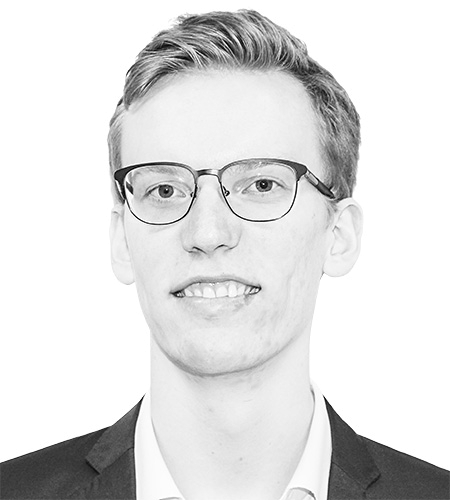
\includegraphics[scale=0.4]{profile}}}
\end{picture}

\begin{tabular}{Dl}
    \textsc{Address:}	&	 Vänortsvägen 5, Luleå, Sweden \\
    \textsc{Phone:}		&	 +46 73 763 87 77\\
    \textsc{email:}		&	 \href{mailto:Claes.Gustaf.Andersson@gmail.com}{Claes.Gustaf.Andersson@gmail.com}\\
    \textsc{Linkdin:}		&	 \url{se.linkedin.com/in/ClaesGustaf}
\end{tabular}

\section{Education}
\begin{tabular}{D L {\textwidth - 2.7cm}}
\textsc{Jun 2018}	&	\textbf{Computer Engineering Master's Degree}\\
\textsc{Aug 2012}	&	 \emph{Information and Communication Technology}. Luleå Tekniska Universitet.\\
			&	Focus on Algorithms, Design paradigms, high levels of abstraction, Networking and Internet services and development.
\end{tabular}


%Section: Work Experience at the top
\section{Work Experience}
\begin{tabular}{D L {\textwidth - 2.7cm}}
 \emph{Current} 	& 	\textbf{Brand Ambassador}	\\
 \textsc{Mar 2014}	&	Academic Work			\\
 			&	{\small Tasked with maintaining and promoting the brand ``Academic Work'' and slogan ``Home of the Young Professional'' on campus. A job requiring effortless socialising with both strangers and colleagues, independent effort but also to be able to work together in tight groups, and to always appear professionally.}	\\
			&						\\
\emph{Current}	&	\textbf{Co-founder}		\\
\textsc{Sep 2013}	&	DC Technological Innovations HB	\\
 			&	{\small A company created in attempts to bring the crypto-currency Bitcoin to our university and make it the dominant payment method within campus. Now mostly idle.  }					\\
 			&						\\
\textsc{Aug 2016}	&	\textbf{Junior Developer}		\\
\textsc{Jul 2016}	&	isMobile				\\
			&	{\small Worked as a consultant through Academic Work. Worked with developing a demo suite for their Android Application Module. Worked primarily in XSLT, HTML, JavaScript and Java}	\\
			

\end{tabular}



%Section: Scholarships and additional info
\section{Scholarships and Certificates}
\begin{tabular}{rl}
 \textsc{Sept.} 2006 & Scholarship for graduate students with an outstanding curriculum \footnotesize(\EURcr 30,000)\normalsize\\
\textsc{June} 2006 & {\textsc{Gmat}\textregistered}\setmainfont[SmallCapsFont=Fontin-SmallCaps.otf]{Fontin.otf}: 730 (\textsc{q:50;v:39}) 96\textsuperscript{th} percentile; \textsc{awa}: 6.0/6.0 (89\textsuperscript{th} percentile)
\end{tabular}

%Section: Languages
\section{Languages}
\begin{tabular}{rl}
 \textsc{Italian:}&Mothertongue\\
\textsc{English:}&Fluent\\
\textsc{French:}&Basic Knowledge\\
\end{tabular}

\section{Computer Skills}
\begin{tabular}{rl}
 Basic Knowledge:& \textsc{php}, my\textsc{sql}, \textsc{html}, Access, \textsc{Linux}, ubuntu, {\fb \LaTeX}\setmainfont[SmallCapsFont=Fontin-SmallCaps.otf]{Fontin.otf}\\
Intermediate Knowledge:& \textsc{vba}, Excel, Word, PowerPoint\\
\end{tabular}

\section{Interests and Activities}
Technology, Open-Source, Programming\\
Paradoxes in Decision Making, Psychoanalysis, Behavioural Finance\\
Football, Travelling

\newpage
\par{\centering\Large \hypertarget{grds}{Master of Science in \textsc{Finance}}\par}\large{\centering Grades\par}\normalsize
\begin{center}
\begin{tabular}{lcc}
\multicolumn{1}{c}{\textsc{Exam}}&\textsc{Grade}&\textsc{Credit Hrs}\\ \hline
Corporate Finance (Valuation)	&25&	6\\
Financial Statement Analysis	&28&	6\\
Statistics	&27&	6\\
Theory of Finance	&26&	6\\
Quantitative Methods for Finance	&30&	6\\
Econometrics	&24	&6\\
Derivatives	&31&	6\\
Management of Financial and Insurance Companies	&30&	6\\
Business Law	&31&	6\\
Investment Banking	&28&	6\\ \\
		
Behavioral Models for Economics and Finance	&29&	6\\
Numerical Methods for Finance	&29&	6\\
Advanced Derivatives	&30&	6\\
Fixed Income (Advanced Methods)	&30&	6\\ \\
		
English Language	&30&	4\\
French Language	&31&	4\\
		
Internship	&	&8\\
		
Final Thesis	&	&20\\
		
		& Total&120\\\cline{2-3}
&\textsc{Gpa}&\textbf{28.61}
\end{tabular}
\end{center}
\bigskip
\hrule
\bigskip
\par{\centering\Large \hypertarget{grds_cleli}{Undergraduate Degree in \textsc{Law and Business Administration}}\par}\large{\centering Grades\par}\normalsize

\begin{center}

\tablefirsthead{%
  \multicolumn{1}{c}{\textsc{Esame (\textsc{ita})}}&\multicolumn{1}{c}{\textsc{Exam (\textsc{eng})}}&\textsc{Grade}&\textsc{Credit Hrs}\\ \hline}
\tablehead{%
\multicolumn{1}{c}{\textsc{Esame (\textsc{ita})}}&\multicolumn{1}{c}{\textsc{Exam (\textsc{eng})}}&\textsc{Grade}&\textsc{Credit Hrs}\\ \hline
}
\tabletail{%
}
\tablelasttail{}	

 \begin{supertabular}{p{4.9cm} p{4.9cm} c c}
Economia aziendale&Theory and principles of management& 28 & 8\\
Istituzioni di diritto privato&Principles of private law&30&8\\
 Istituzioni di diritto pubblico 
&
 Principles of public law 
& 30&
 6 
\\
Matematica generale 
& Mathematics 
&31&8\\
 Contabilit\`a e Bilancio 
& Accounting and Financial statements 
& 31 & 8\\
 Diritto del lavoro 
&
 Labour law 
& 30&
4 
\\
 Informatica & Computer skills &29& 4 
\\
 Economia e gestione delle imprese & Corporate management &31&6 
\\
 Microeconomia & Microeconomics &30&8 
\\
 Contabilit\`a e bilancio 2 & Accounting and financial statements 2 
&29&8 \\
 Diritto commerciale & Company and business law &30&8 
\\
 Macroeconomia & Macroeconomics &29&8 
\\
 Statistica & Statistics &30&6\\
 Diritto delle procedure concorsuali & Insolvency law &31&4 
\\
 Finanza aziendale 
& Corporate finance 
&31 &8 \\
 Matematica finanziaria & Financial mathematics &31&4 
\\
 Programmazione e controllo 
& Management accounting &31&8 
\\
Lingua Inglese \textsc{c1}& English Language \textsc{c1}& 25&6\\ 
Diritto tributario & Tax law &30&6 
\\
Organizzazione e sistemi informativi aziendali &Management information systems &28&6 
\\
 Strategia e politica aziendale* 
& Business strategy* & 29& 6 
\\
Derivati*&Derivatives*&30&6\\
Opzionale all'estero* & Corporate Financial Strategy* &30&6\\
Lingua Francese \textsc{b1} & French Language \textsc{b1}&31&6\\
Economia dei mercati e degli intermediari finanziari* 
&Financial markets and institutions* &30&6 
\\
Revisione aziendale 
&Financial auditing &31&6 
\\
Scienza delle finanze &Public economics &30&6 
\\
 Lavoro finale& Final report&&6\\
& & Total&180\\\cline{3-4}
& &\textsc{Gpa}&\textbf{29.85}\\ \\ \multicolumn{4}{l}{\footnotesize A star (*) indicates that the course was taken at the \textbf{University of Southern California}, Los Angeles, \textsc{usa}}
 \end{supertabular}
\end{center}
\bigskip
\hrule
\bigskip
\par{\centering\Large \hypertarget{grds_usc}{Exchange Program at \textsc{usc}, Los Angeles}\par}\large{\centering Grades\par}\normalsize

\begin{center}
\begin{tabular}{lcc}
\multicolumn{1}{c}{\textsc{Exam}}&\textsc{Grade}&\textsc{Grade Points}\\ \hline
Corporate Financial Strategy	&A&	4\\
Derivatives	&A&	4\\
Money, Credit, and Banking	&A&	4\\
Business Strategy & A-& 3.5\\
& &\\\cline{2-3}
 &\textsc{Gpa}&\textbf{3.875}
\end{tabular}
\end{center}
%\newpage
%\hypertarget{gmat}{\textsc{Gmat}\setmainfont{LMRoman10 Regular}\textregistered\setmainfont[SmallCapsFont=Fontin-SmallCaps]{Fontin-Regular}}

%\XeTeXpdffile ''GMAT.pdf'' page 1 scaled 800

\end{document}
